
\chapter{LITERATURE REVIEW}
\label{chap:literature-review}
\thispagestyle{fancy}
(Sub-chapter mentioned below is for typing guidelines only. Discuss with your advisor for the actual sub-chapter title and content). It is advisable (not-compulsory) to write introductory sentences here prior to further elaboration in the sub-chapter. The sub-chapter mentioned here serves as samples, and should not be considered as compulsory. Contact your thesis adviser for the actual sub-chapter division.
	 
\section{Theoretical Perspectives}
\label{sec:theoretical-perspective}
This is the body of your thesis. Please check that your body of thesis consistency in term of font type, font size, spacing, and margin are maintained \cite{gdbusecaseneo4j}. This is the body of your thesis. Please check that your body of thesis consistency in term of font type, font size, spacing, and margin are maintained. This is the body of your thesis \cite{linuxstatistic}. Please check that your body of thesis consistency in term of font type, font size, spacing, and margin are maintained \cite{shin2022focusing}.

\begin{figure}[htbp]
	\centering 
	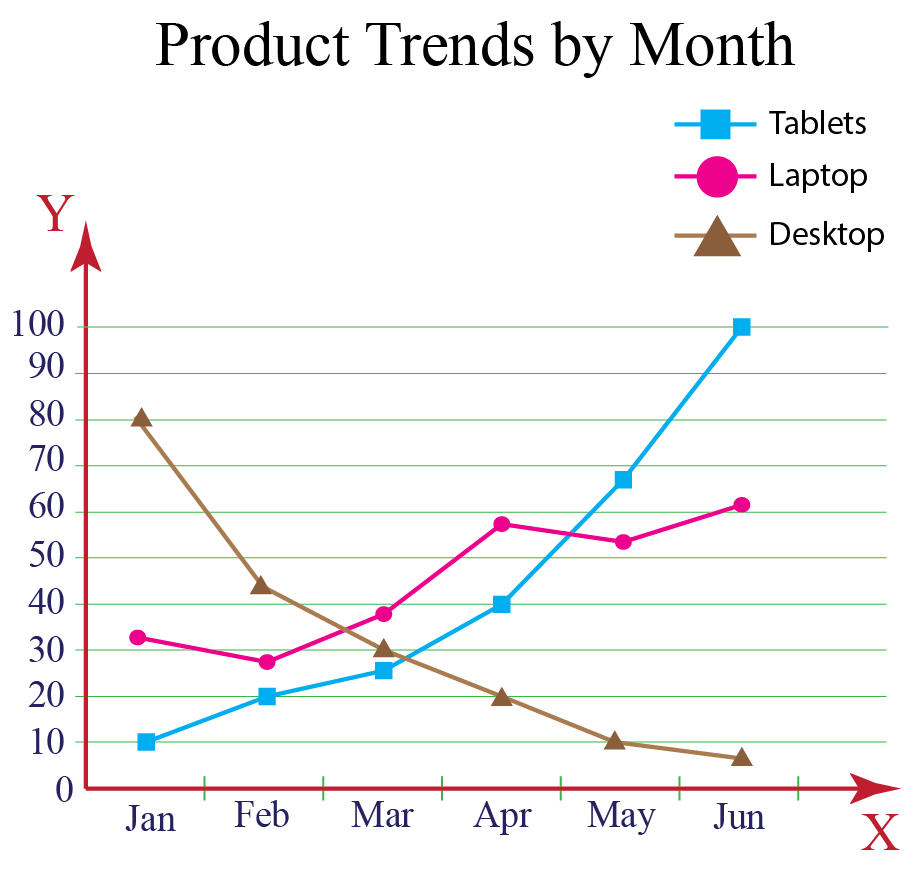
\includegraphics[width=0.6\textwidth]{images/graph.png}
	\caption{Another example of figure placement in your body of thesis and its label}
	\label{fig:figure-example}
\end{figure} 
 
Figure \ref{fig:figure-example} is ....

This is the body of your thesis. Please check that your body of thesis consistency in term of font type, font size, spacing, and margin are maintained \cite{djap_xb_pot}. This is the body of your thesis. Please check that your body of thesis consistency in term of font type, font size, spacing, and margin are maintained \cite{cabral2019review}. This is the body of your thesis \cite{boffa2022towards}. Please check that your body of thesis consistency in term of font type, font size, spacing, and margin are maintained \cite{exabeam}.This is the body of your thesis. Please check that your body of thesis consistency in term of font type, font size, spacing, and margin are maintained.This is the body of your thesis. Please check that your body of thesis consistency in term of font type, font size, spacing, and margin are maintained. This is the body of your thesis. Please check that your body of thesis consistency in term of font type, font size, spacing, and margin are maintained.

Please note that all figures and graphs in the body of thesis are in grayscale, unless really necessary. Color printed material can be placed as appendix. Cite it as  \ref{fig:figure-example}

\section{Previous Studies}
\label{sec:previous-studies}
I want to cite a paper from \cite{shrivastava2019attack}, because ... \\

This is the body of your thesis. Please check that your body of thesis consistency in term of font type \cite{honeypot_spitzner}, font size, spacing, and margin are maintained. This is the body of your thesis. Please check that your body of thesis consistency in term of font type \cite{noor2019machine}, font size, spacing, and margin are maintained.

\begin{table}
	\centering
	\caption{Example of Comparison Table}
	\begin{tabularx}{\linewidth}{X c X X}
			\hline
			\textbf{No} & \textbf{Paper} & \textbf{Description} \\ 
			\hline
			Feature number 1 & 1 & This is the description of what you want to explain, please elaborate in a clear and concise sentence & Sesuatu \\
			Feature number 2 & 2 & This is the description of what you want to explain, please elaborate in a clear and concise sentence & Sesuatu \\
			Feature number 3 & 3 & This is the description of what you want to explain, please elaborate in a clear and concise sentence \\
			Feature number 4 & 4 & This is the description of what you want to explain, please elaborate in a clear and concise sentence & Sesuatu \\
			\hline
	\end{tabularx}
	\label{tab:example-of-comparison-table}
\end{table}

This is the body of your thesis. Please check that your body of thesis consistency in term of font type, font size, spacing, and margin are maintained. This is the body of your thesis. Please check that your body of thesis consistency in term of font type, font size, spacing, and margin are maintained. This is the body of your thesis. Please check that your body of thesis consistency in term of font type, font size, spacing, and margin are maintained.

Please make sure that you use consistent style of table throughout your body of thesis. This is the body of your thesis. Please check that your body of thesis consistency in term of font type, font size, spacing, and margin are maintained. This is the body of your thesis. Please check that your body of thesis consistency in term of font type, font size, spacing, and margin are maintained.
